\section{硬件生态与无线通信拓扑}
\label{sec:hardware}

\subsection{板端主机与外设}

本项目的板端主机使用 RK3399ProX 开发板。它承担本地服务、状态机、
Web 前端、语音守护进程和部分视觉推理任务，也是各类传感数据最终汇合的
节点。板端外设主要包括摄像头、麦克风、扬声器或外接音箱，以及 Web 网页
展示所需的网络入口。这样的组合优先保证多路输入能够稳定汇聚，并让
训练状态、传感状态和调试信息可以被直接观察。

\begin{figure}[htbp]
    \centering
    \includegraphics[width=0.92\textwidth]{figures/report/fig02-board.png}
    \caption{RK3399ProX 板端主机及外设连接实拍。}
    \label{fig:board-photo}
\end{figure}

摄像头负责提供视觉姿态估计输入，麦克风和扬声器负责语音交互，Web 前端
则承担训练状态、肌电波形、模式信息和调试入口的展示。把这些外设接到同一
板端后，系统不再是几个独立功能的拼接，而是可以围绕一次训练流程组织
输入、判断和反馈。

\subsection{ESP32 肌电传输单元}

肌电侧由贴片电极、肌电采集模块、ESP32 主控和电源组成。贴片电极贴在
目标肌和可能代偿的肌群附近，采集模块完成模拟前端处理，ESP32 负责读取
通道值并通过无线链路发送到板端。这个单元的设计重点是把采集、供电、
无线传输和佩戴固定组织成一条可连续工作的传感链路。

\begin{figure}[htbp]
    \centering
    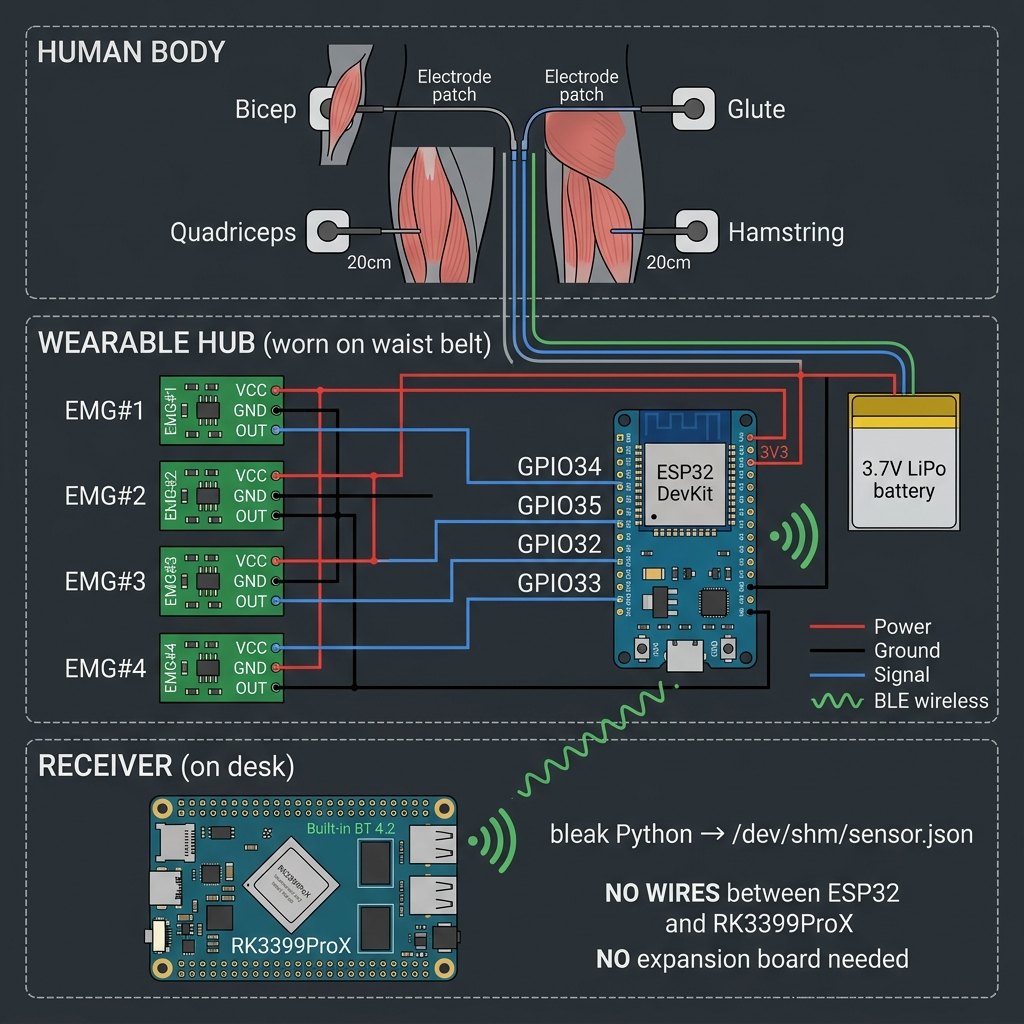
\includegraphics[width=0.72\textwidth]{figures/report/fig03-unit.jpg}
    \caption{肌电采集与传输单元早期结构示意。}
    \label{fig:wearable-concept}
\end{figure}

肌电信号幅值很小，对接地、布线和贴片稳定性都比较敏感。项目后期的方向是
把采集板、ESP32 主控和电源进一步集中到一块自制集成板中，再通过更短的
线路引出到目标肌群。这样做有三个好处：装配时少接线、运动时线束更短、
电源和信号路径更容易固定。对可穿戴设备来说，这不仅是美观问题，也关系到
佩戴安全和信号稳定。

\subsection{穿戴结构与走线}

硬件佩戴方式同样影响系统可用性。最直接的做法是把板子和电极都固定在手臂
或腿上，但实际运动时会遇到两个问题：一是线束容易随动作摆动，二是贴片
受到拉扯后会改变接触状态。项目最终采用更稳妥的穿戴思路：主机、电池和
ESP32 放在腰包或贴身固定区域，贴片只通过短线连接到目标肌群；运动服和
肩带用于固定线路，让设备不影响深蹲、弯举等动作。

\begin{figure}[htbp]
    \centering
    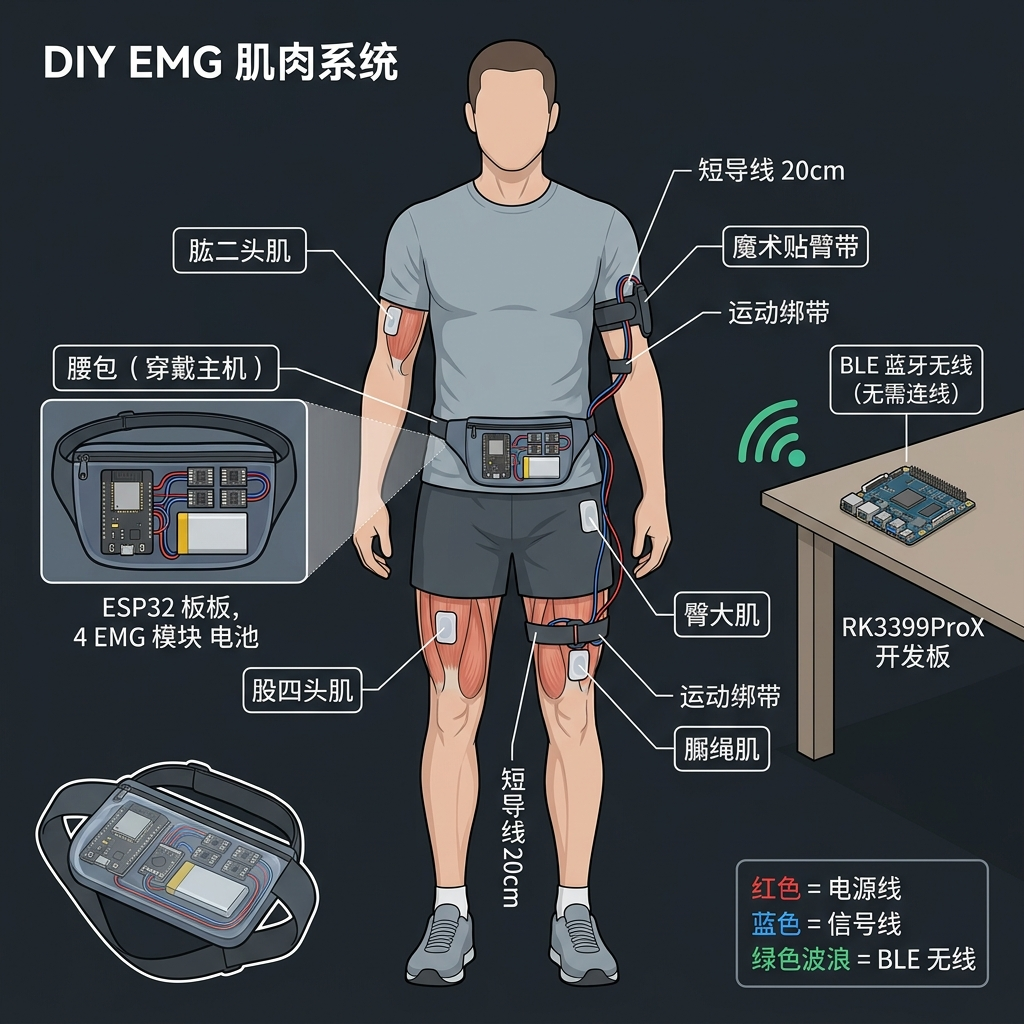
\includegraphics[width=0.85\textwidth]{figures/report/fig03-system.jpg}
    \caption{DIY 肌电系统整体穿戴示意：腰包集中放置 ESP32 主控、4 路 sEMG 采集模块和电池，贴片经短导线连接目标肌群，BLE/Wi-Fi 上行至 RK3399ProX 板端。}
    \label{fig:wearable-routing}
\end{figure}

这种结构的优点是把重量放在身体更稳定的位置，同时把敏感的电极线尽量贴近
身体走线。它还方便调试：需要更换贴片位置时，不必重新拆整套主机；需要
观察板端状态时，也可以直接从腰包或工作台取出模块。相比把多个模块分散
固定在四肢上，腰包和短线结构更容易控制重量分布和线束拉扯。

\subsection{从 BLE 到 Wi-Fi UDP}

无线通信路线保留了项目里的一个真实转折。早期使用 BLE，是因为它低功耗、
资料多，也符合可穿戴设备的常见直觉。但肌电信号不是偶尔上报一次的状态量，
而是连续变化的时序数据。通道数和采样频率提高以后，BLE 的连接间隔、握手
和吞吐限制逐渐影响连续数据流。

项目最终改用 Wi-Fi UDP。ESP32 不再维护复杂连接状态，而是把每帧肌电特征
封装成 UDP 数据报发给 RK3399ProX。UDP 没有重传和确认机制，表面上不如
可靠传输完整；但对于滑动窗口和动作周期分析来说，偶尔丢失一个瞬时点通常
比整条反馈链路持续堆积延迟更容易处理。健身反馈更需要连续、轻量、能容忍偶发丢点
的数据流，而不是把所有历史包都排队补齐。

\begin{figure}[htbp]
    \centering
    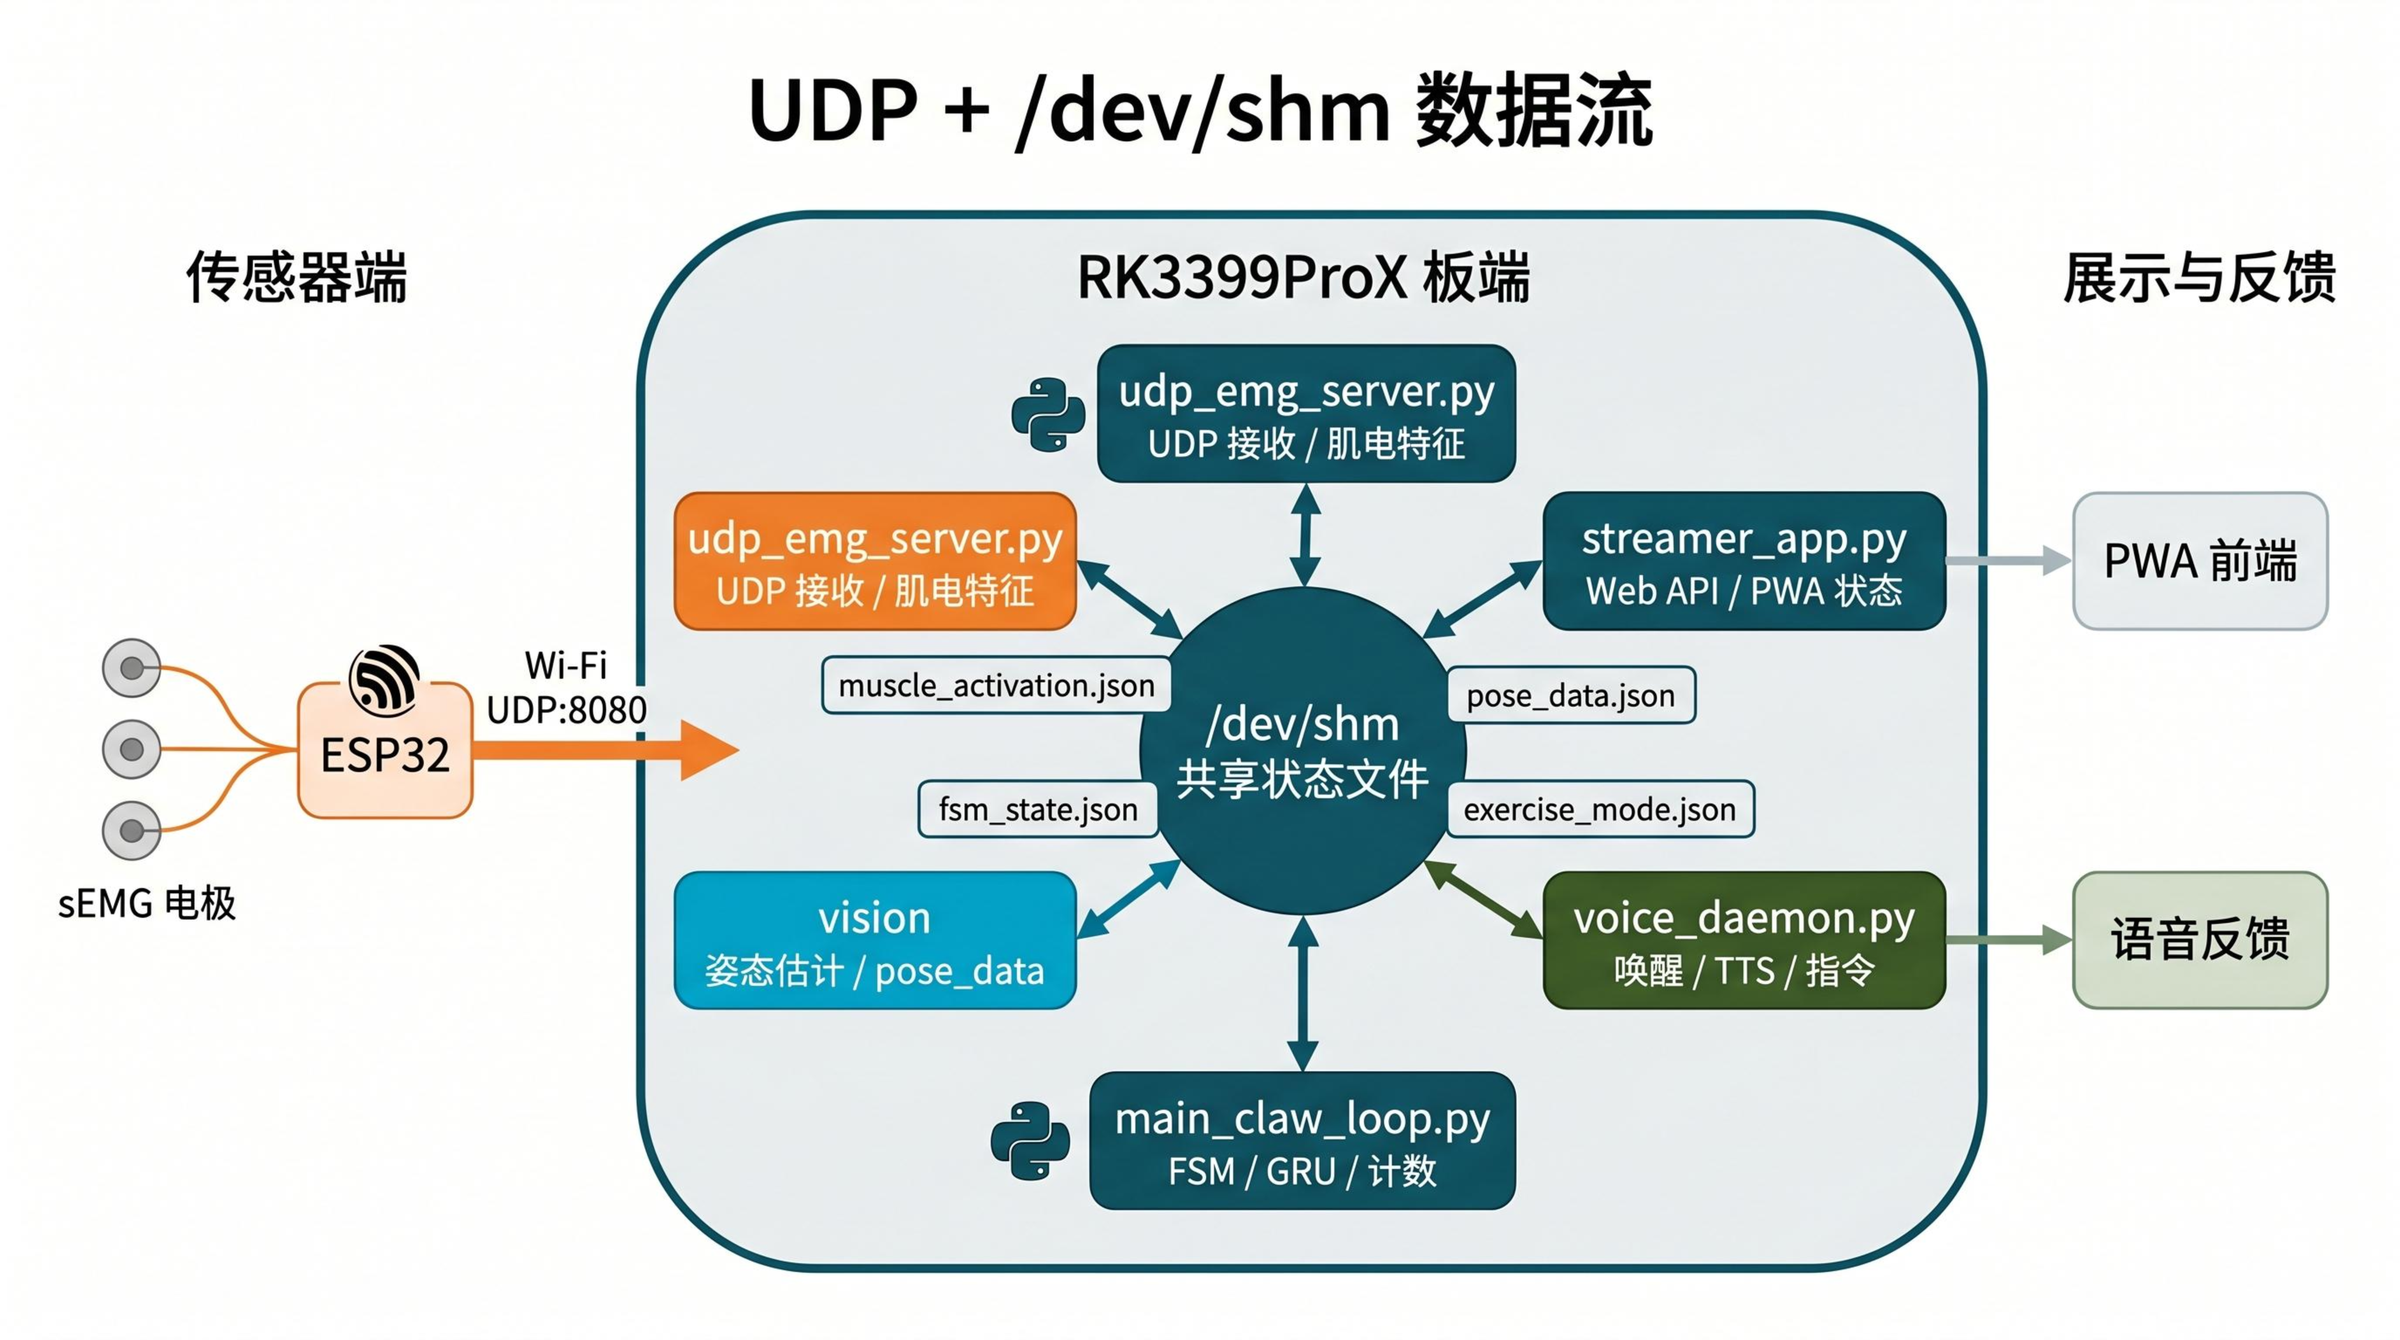
\includegraphics[width=0.92\textwidth]{figures/report/fig04.png}
    \caption{肌电数据从 ESP32 进入板端后的通信与共享状态文件流向。}
    \label{fig:udp-shm-dataflow}
\end{figure}

\subsection{硬件结构与集成方向}

采集板的原理图和 PCB 布局反映了接口、电源、固定孔和模拟/数字区域的
基本关系。完整电路细节以源文件为准，正文主要关注采集、传输和佩戴结构
之间的系统关系。

\begin{figure}[htbp]
    \centering
    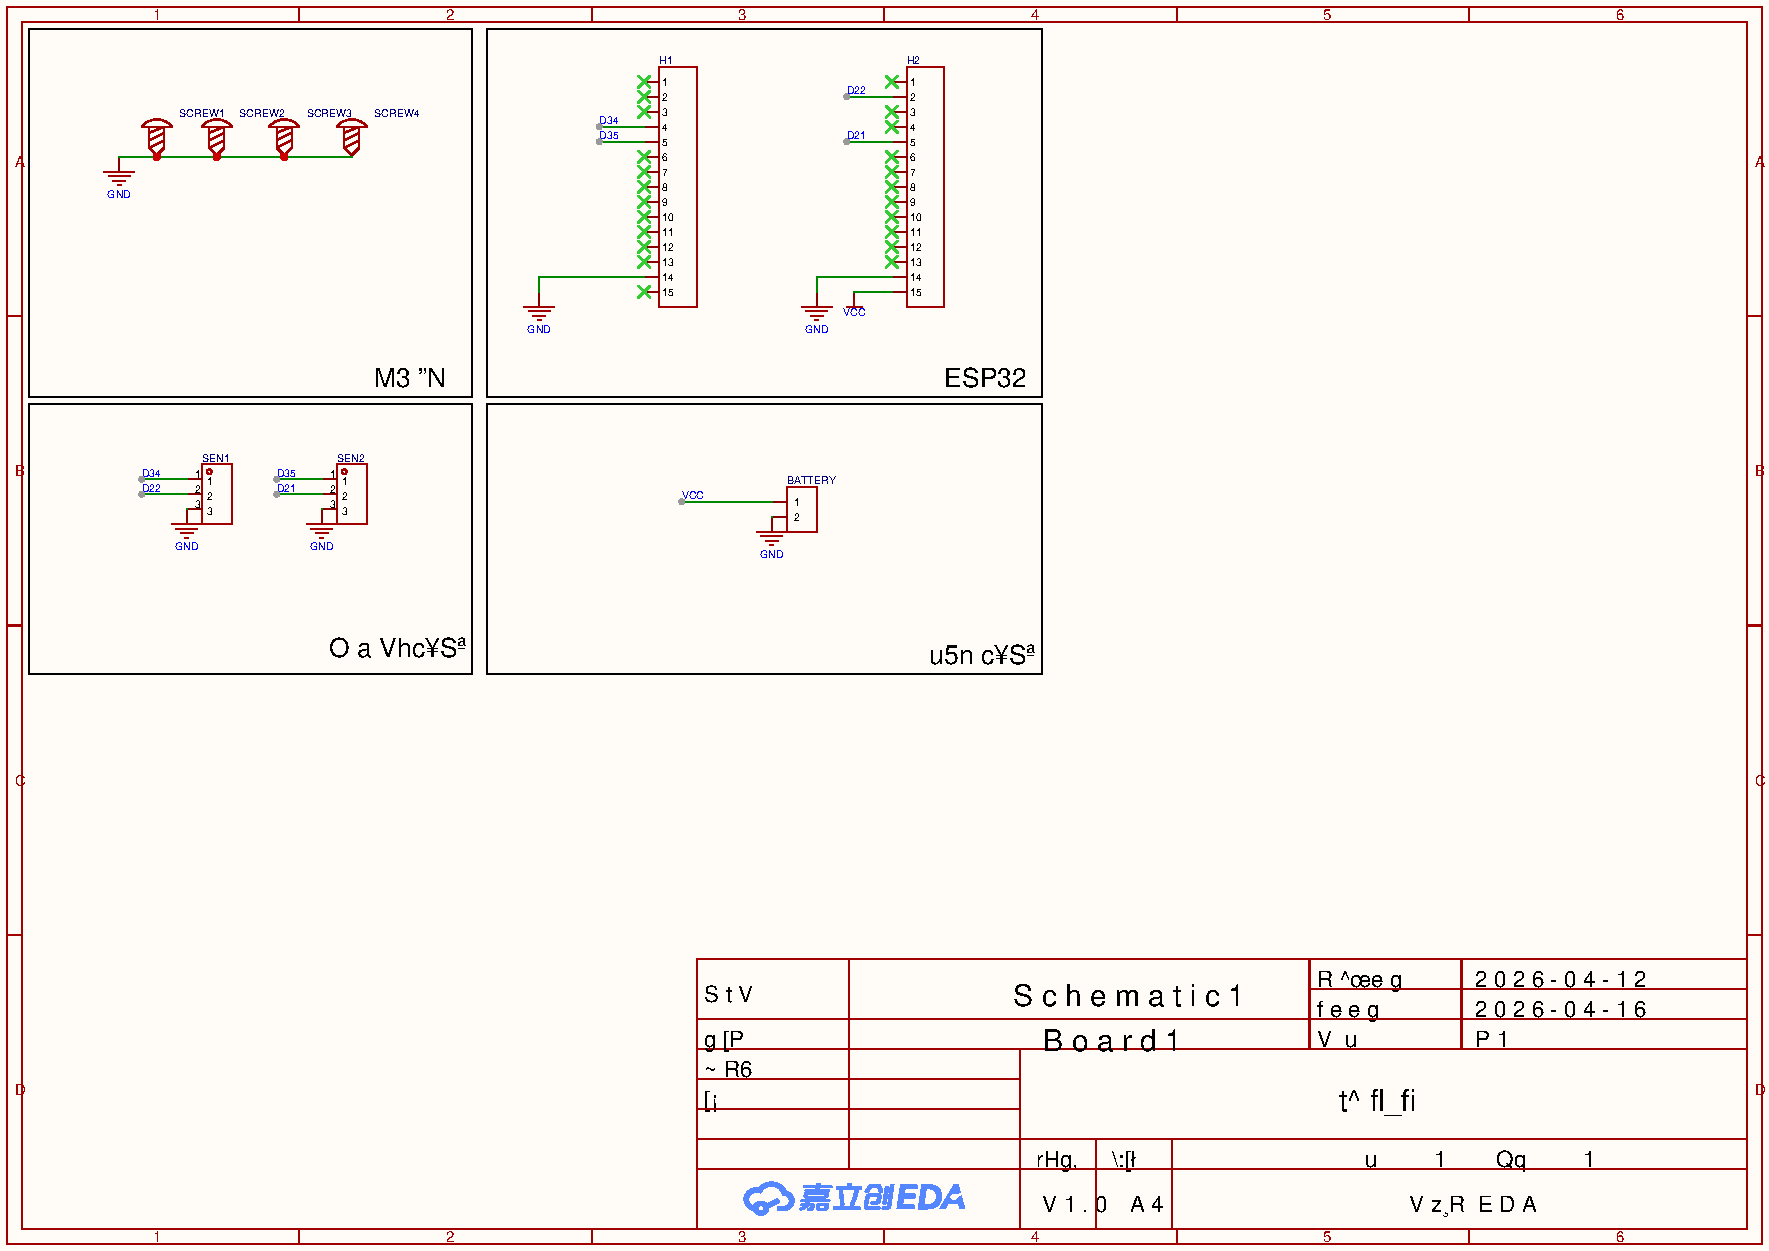
\includegraphics[width=0.94\textwidth]{figures/report/hw01.pdf}
    \caption{肌电采集板原理图概览。}
    \label{fig:hardware-schematic}
\end{figure}

\begin{figure}[htbp]
    \centering
    \includegraphics[page=4,width=0.42\textwidth]{figures/report/hw02.pdf}
    \caption{肌电采集板 PCB 局部布局。}
    \label{fig:hardware-pcb}
\end{figure}

